\chapter{Anexo D}
\label{cap:AnexoD}

En este anexo se muestra el manual de usuario de la aplicación de este documento mediante capturas de pantalla de la solución, acompañadas de una descripción.

\subsection{Inicio de sesión}
Se ha desarrollado una ventana para que el usuario inicie sesión (ver figura \ref{Fig:login}). Es la primera ventana que se encuentra al ejecutar el programa.

\begin{figure}[h]
\centering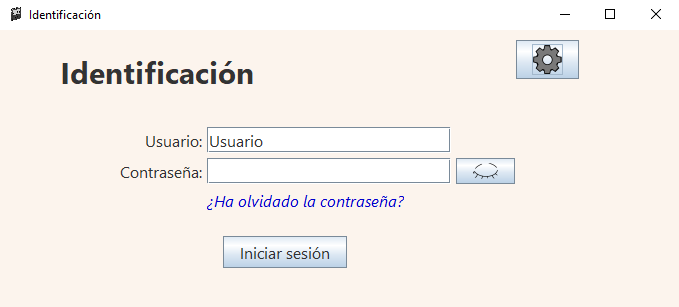
\includegraphics[width=1\linewidth]{figs/login.png}
\caption{Pantalla de inicio de sesión.}
\label{Fig:login}
\end{figure}

Esta ventana permite al usuario acceder a las opciones del programa haciendo clic en la rueda de opciones, e iniciar sesión en la aplicación con su DNI y una contraseña asociada. En la figura \ref{Fig:loginopciones} se pueden ver las diferentes opciones de adaptación a las necesidades del usuario que se ofrecen:
\begin{itemize}
	\item \textbf{Cambio del tamaño de la letra}, seleccionando entre 5 diferentes tamaños de letra.
	\item \textbf{Colores para las notas aprobadas, suspensas y el fondo de la aplicación}. Hay también 5 opciones para los colores de las notas, que son colores sólidos y fuertes, y otras 5 para el fondo, colores pastel que permiten el contraste de los demás elementos de la ventana.
	\item \textbf{Modo oscuro}. Este modo modifica toda la interfaz gráfica, cambiando el contraste con un fondo negro y letras blancas. Esta opción de diseño se llevó a cabo debido a que a medida que va pasando el tiempo, el 'modo nocturno' o 'modo oscuro' de los dispositivos y aplicaciones se vuelve más popular.
	\item \textbf{Modo daltónicos}. Este modo bloquea la posibilidad de cambiar los colores de aprobados y suspensos, poniendo dos colores que son fácilmente distinguibles para la mayoría de personas con daltonismo.
\end{itemize}

\begin{figure}[h]
\centering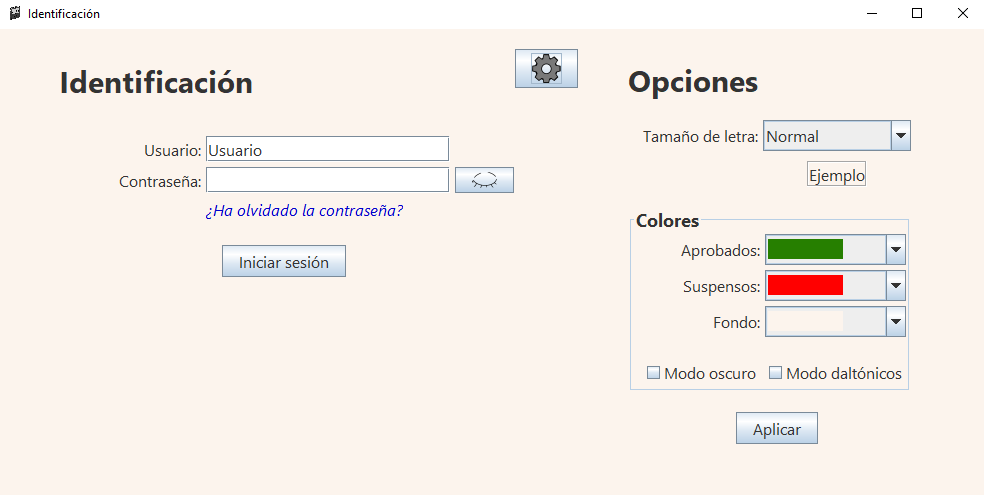
\includegraphics[width=1\linewidth]{figs/loginopciones.png}
\caption{Pantalla de inicio de sesión con opciones.}
\label{Fig:loginopciones}
\end{figure}

Esta ventana también contiene un botón con un ojo cerrado que, al hacerle clic, se abre y muestra la contraseña, y una opción de recuperado de contraseña por si el usuario se olvidara de ella.


\subsection{Ventana principal}
Esta ventana es el centro de operaciones de la aplicación, y desde aquí se puede navegar a todas sus características y funcionalidades, de las que se habla en las siguientes secciones. Esta ventana se puede ver en la figura \ref{Fig:ventanaprincipal}.

\begin{figure}[h]
\centering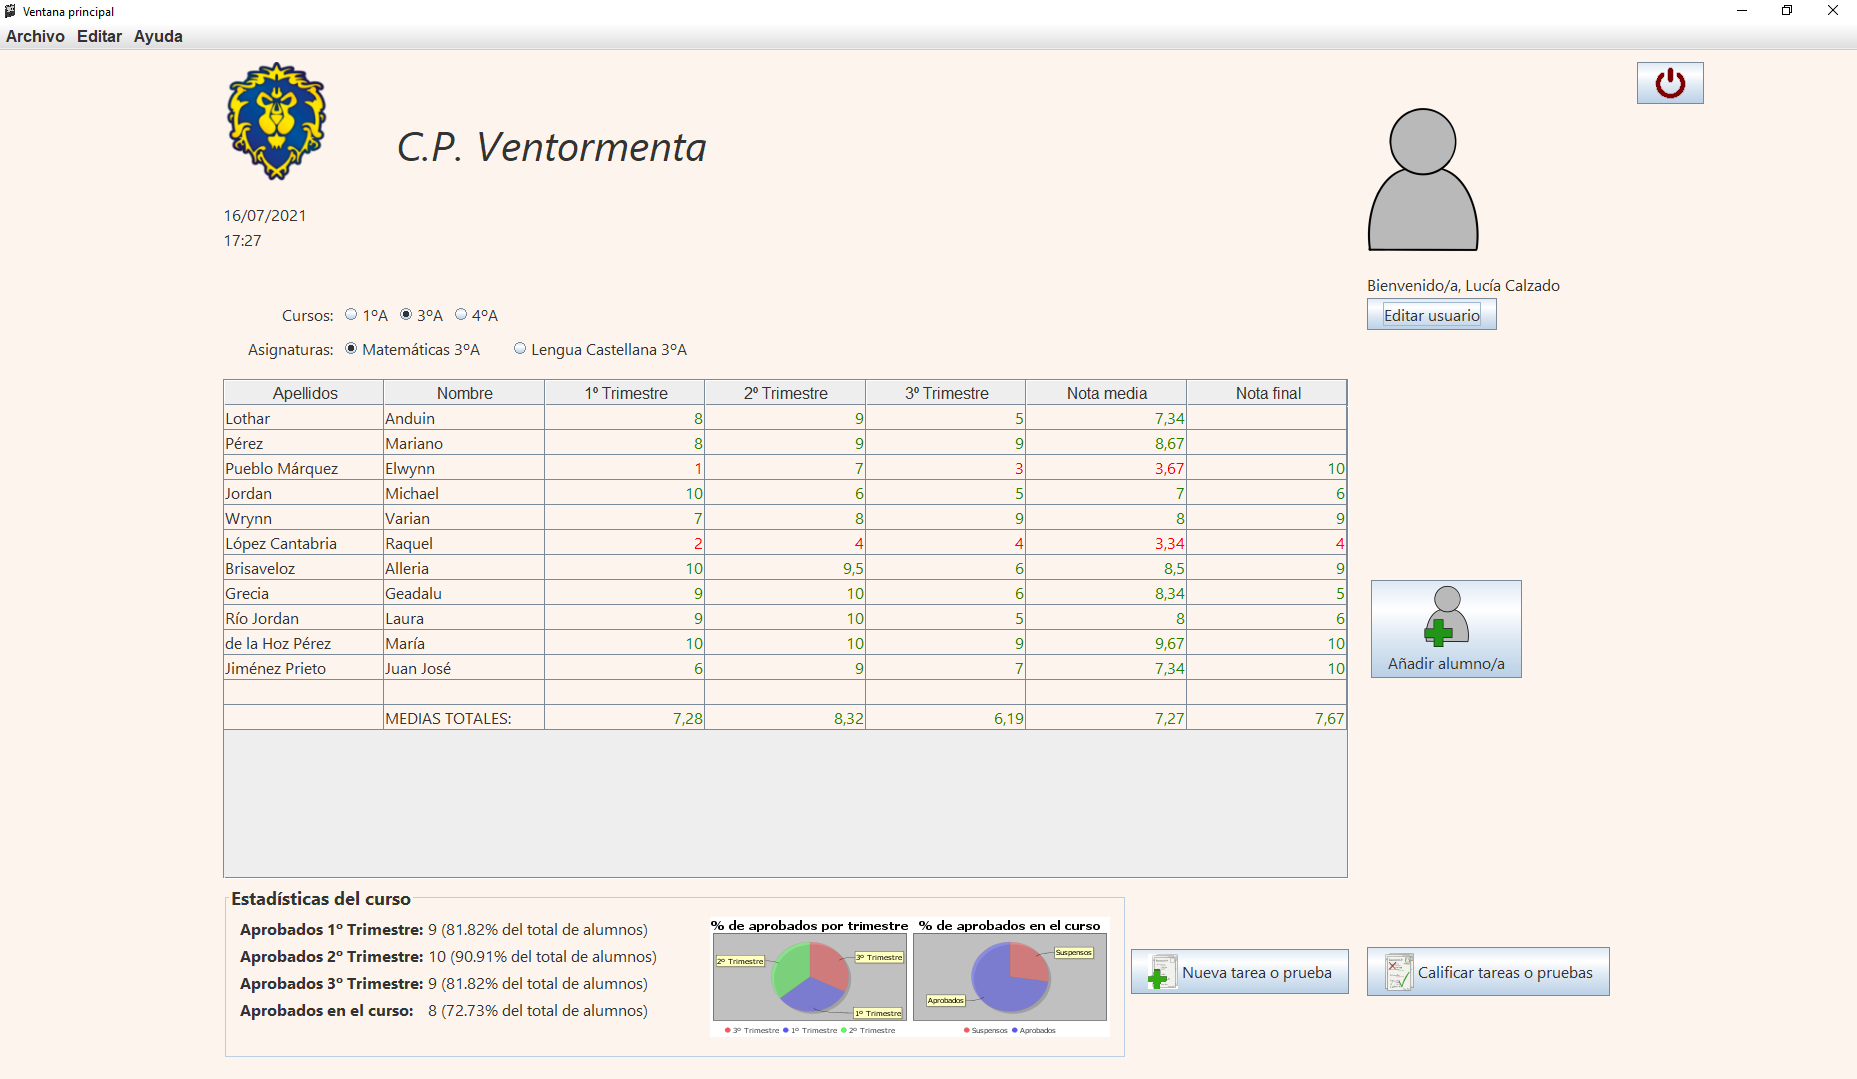
\includegraphics[width=1\linewidth]{figs/ventanaprincipal.png}
\caption{Ventana principal de la aplicación.}
\label{Fig:ventanaprincipal}
\end{figure}

En el menú de arriba se puede cerrar sesión en Archivo>Cerrar sesión, añadir un alumno o varios desde el menú Editar>Alumnos y acceder al manual de ayuda en Ayuda>Manual de ayuda, así como visualizar una pequeña ventana 'Acerca de...' que muestra los datos personales de la desarrolladora de este trabajo.

En la parte de arriba de la ventana vemos el logotipo y el nombre del Centro que está usando la aplicación, así como la fecha y la hora del día actual. 

En el centro, el usuario puede elegir el curso y la asignatura para los que desea hacer los trámites, y aparece una tabla con los alumnos asignados y sus notas finales para cada trimestre, una nota media de los tres trimestres y una nota final. Cabe notar que las notas tienen colores (que se pueden personalizar en las opciones de la ventana de Inicio de sesión) dependiendo de si el trimestre está aprobado o suspenso. El usuario también puede consultar la fecha de cierre de actas para cada trimestre manteniendo el ratón por encima del nombre de cada trimestre en la tabla. Esta información se muestra mediante un \textit{tooltip}.

En la última fila de la tabla también hay un cálculo de medias, esta vez por trimestre y no por alumno.

Debajo de la tabla se ven las estadísticas de la asignatura: el número de aprobados por trimestre y en total en el curso, así como dos diagramas de quesitos mostrando los datos mencionados anteriormente: uno para los aprobados por cada trimestre, para representar de manera visual qué trimestre ha sido el más exitoso, y uno de los alumnos aprobados en todo el curso, para representar el éxito del curso en general.

A la derecha de estas estadísticas están los accesos a las funcionalidades de crear una nueva tarea y calificar a los alumnos en las tareas existentes, así como la de añadir un alumno nuevo a la asignatura.

Por último, arriba a la derecha se encuentran los datos del maestro: su nombre y su fotografía, y el acceso a la funcionalidad de modificar los datos del usuario, así como el botón de cerrar sesión, arriba a la derecha.


\subsection{Editar usuario}
Mediante el botón Editar usuario en la pantalla principal, se accede a la ventana de modificar los datos del usuario: el nombre mediante el que se dirige a él la aplicación, una fotografía personal y la contraseña de inicio de sesión. Esta ventana se puede ver en la figura \ref{Fig:datospersonales}.

\begin{figure}[h]
\centering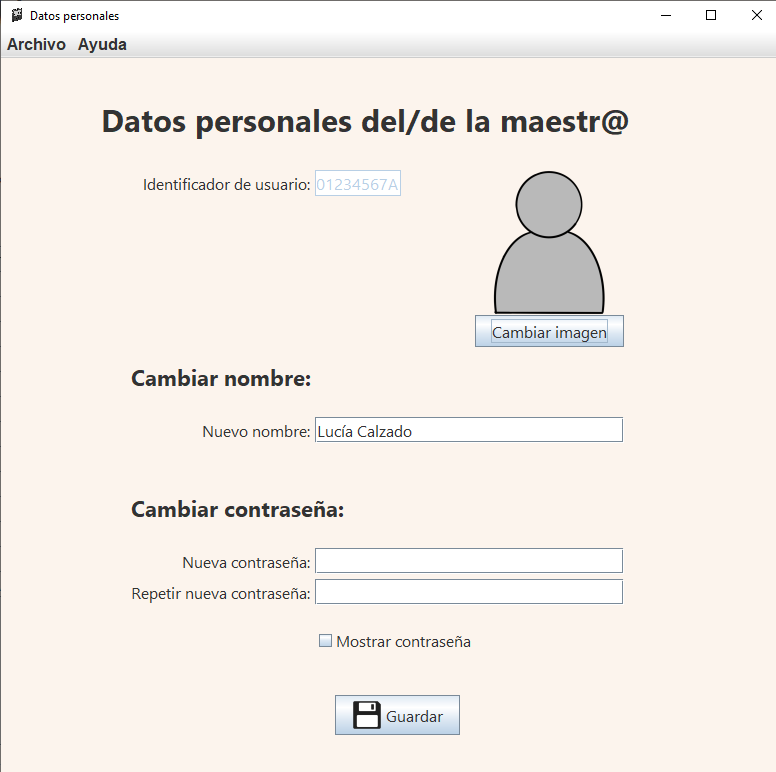
\includegraphics[width=0.5\linewidth]{figs/datospersonales.png}
\caption{Ventana para modificar los datos personales del usuario.}
\label{Fig:datospersonales}
\end{figure}

\subsection{Añadir alumno}
La aplicación permite añadir alumnos de dos maneras. Se puede añadir un solo alumno rellenando un formulario (ver figura \ref{Fig:añadiralumno}), accesible tanto el botón Añadir alumno/a como en el menú Editar>Alumnos de la ventana principal.

\begin{figure}[h]
\centering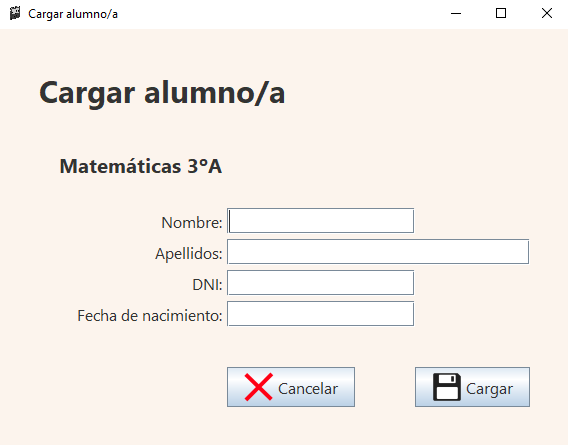
\includegraphics[width=0.5\linewidth]{figs/cargaralumno.png}
\caption{Formulario para añadir un alumno.}
\label{Fig:añadiralumno}
\end{figure}

La segunda opción es añadir varios alumnos cargando un Excel con sus datos: nombre, apellidos, DNI y fecha de nacimiento. Esta opción es únicamente accesible en la ventana principal, mediante el menú Editar>Alumnos.

La aplicación añade los alumnos teniendo en cuenta la asignatura desde la que se ha llamado la funcionalidad. Si la asignatura es troncal, quiere decir que los alumnos están siendo asignados a un curso entero, porque las asignaturas troncales son de carácter obligatorio. Si, por el contrario, son añadidas a una asignatura optativa, solo se añadirán a esa asignatura optativa, no al curso, debido a que las asignaturas optativas son opcionales.

\subsection{Crear nueva tarea}
Una de las dos funcionalidades principales de la aplicación es la de crear una tarea (o prueba) nueva (ver figura \ref{Fig:creartarea}). Esta característica es accesible mediante el botón 'Nueva tarea o prueba' de la ventana principal, una vez se ha seleccionado una asignatura.

\begin{figure}[h]
\centering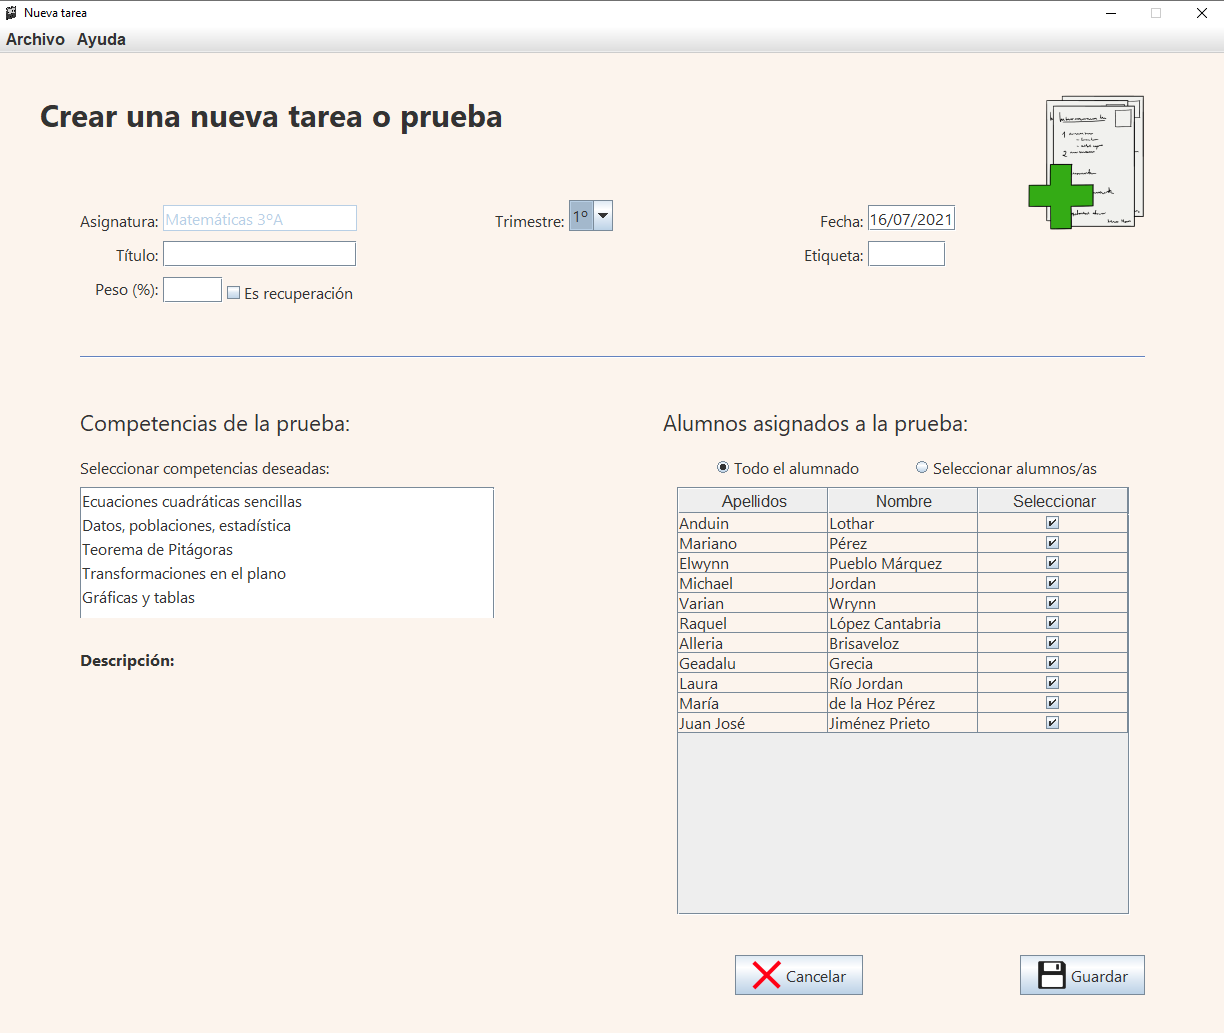
\includegraphics[width=1\linewidth]{figs/creartarea.png}
\caption{Formulario para crear una tarea (o prueba) nueva.}
\label{Fig:creartarea}
\end{figure}

La ventana consta de un formulario que tiene que rellenar el usuario para crear una tarea nueva. A continuación se muestra una breve descripción de los campos:
\begin{itemize}
	\item \textbf{Título:} este es el título que tiene la prueba, usado para consultar las notas en el módulo Calificar tareas o pruebas.
	\item \textbf{Trimestre:} el trimestre para el que se crea la prueba. Es importante para posterior ordenación y muestra de las pruebas por trimestres.
	\item \textbf{Peso:} el peso de la prueba dentro del trimestre, o el porcentaje de la nota final del trimestre que corresponde a esa prueba.
	\item \textbf{Fecha:} la fecha en la que se llevará a cabo la prueba.
	\item \textbf{Etiqueta:} un pequeño título único para la prueba. Debe tener como máximo 5 caracteres.
	\item \textbf{Competencias:} se deben seleccionar las competencias asignadas a la prueba de la lista de competencias. En el apartado Descripción, salen las descripciones asignadas a cada competencia.
	\item \textbf{Alumnos asignados:} debido a que algunas pruebas podrían no ser opcionales o ser exámenes de recuperación, se pueden elegir los alumnos a los que se les quiere asignar la prueba.
\end{itemize}

Cuando se hace clic en el botón de guardar, la prueba se almacena en la base de datos con los datos del formulario.


\subsection{Calificar tareas}
La segunda de las funcionalidades principales de la aplicación es la de calificar las tareas creadas mediante el módulo anterior (ver figura \ref{Fig:calificartarea}). Para acceder a este módulo, se debe hacer clic en el botón 'Calificar tareas o pruebas' de la ventana principal, una vez se ha seleccionado una asignatura.

\begin{figure}[h]
\centering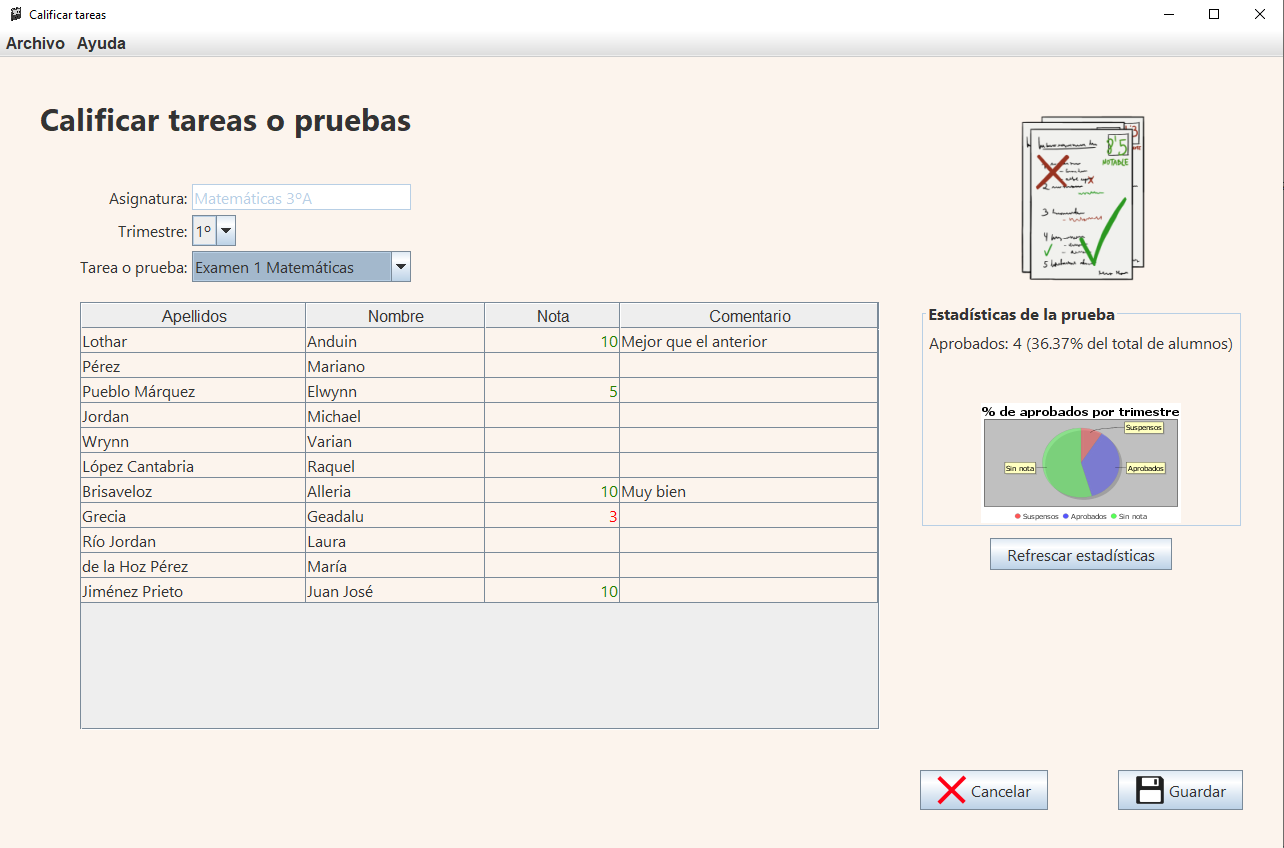
\includegraphics[width=1\linewidth]{figs/calificartareas.png}
\caption{Ventana para calificar las tareas (o pruebas) creadas.}
\label{Fig:calificartarea}
\end{figure}

En esta ventana, se puede elegir el trimestre de la prueba que se va a calificar, y después la misma prueba. Esto cargará una tabla con todos los alumnos de la asignatura, una columna para calificarlos y otra para asignarles un comentario, si el docente considera oportuno.

Si un alumno no tiene que realizar una prueba, por defecto, en el comentario saldrá escrito \textit{"No tiene que hacer la prueba."}. 

A la derecha de la tabla se puede observar otro panel de estadísticas, que muestran el porcentaje de alumnos aprobados en la prueba.

Cuando se haya calificado a los alumnos, al hacer clic en el botón de guardar, se guardarán los cambios en la base de datos.

\subsection{Informe del alumno}
Esta ventana muestra todas las notas, tanto de pruebas como finales, de un alumno en particular (ver figura \ref{Fig:informealumno}). Es accesible haciendo clic en el nombre o apellidos de un alumno en la tabla de la ventana principal.

\begin{figure}[h]
\centering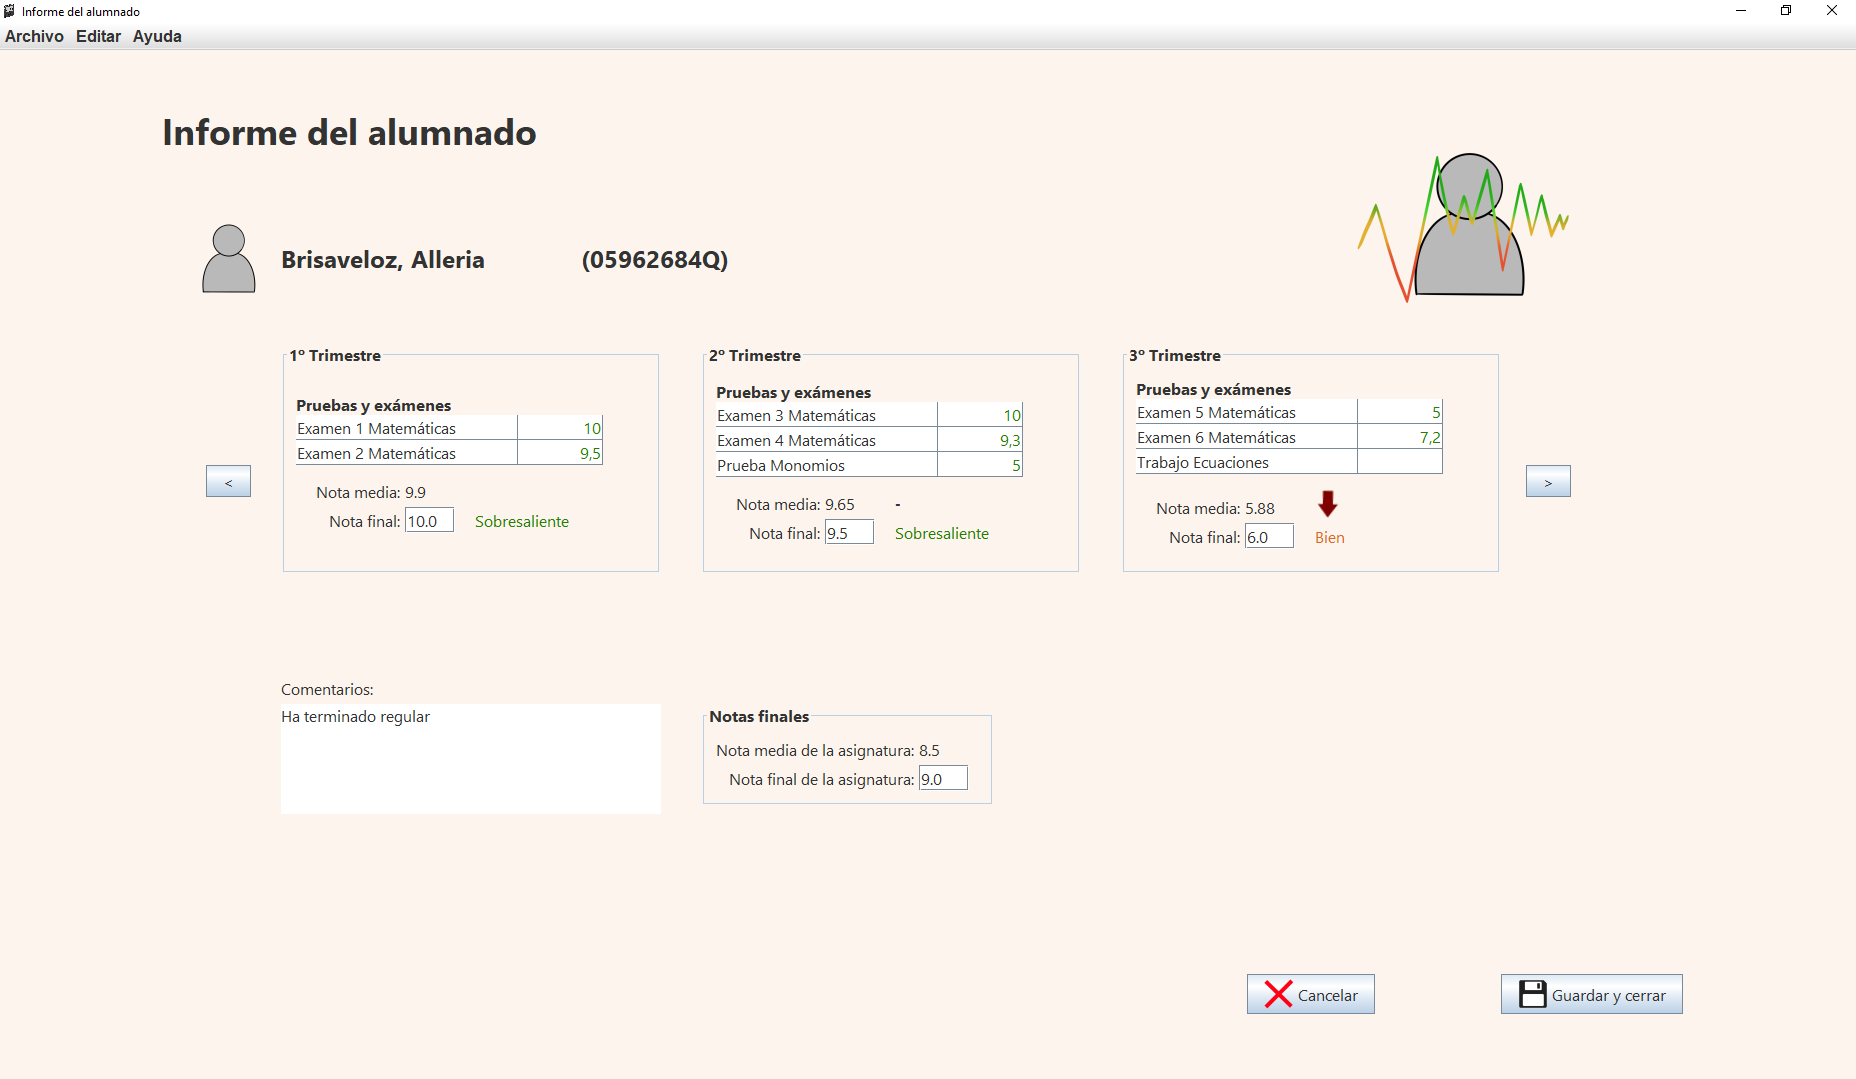
\includegraphics[width=1\linewidth]{figs/informealumno.png}
\caption{Ventana del informe general del alumno.}
\label{Fig:informealumno}
\end{figure}

En la parte de arriba está el nombre y apellidos del alumno, así como su DNI y su fotografía personal.

En el centro de la ventana hay tres tablas que corresponden a los tres trimestres. Cada tabla contiene todas las pruebas de ese trimestre, junto con la nota del alumno. Si se deja el ratón por encima de la nota, se muestra el comentario (si lo hubiera), de la misma mediante un \textit{tooltip}. Debajo de la tabla aparece la media de las notas de las pruebas y la nota final de ese trimestre.

La característica más interesante de esta ventana es la información que se obtiene de cada trimestre:
\begin{itemize}
	\item{Color de las notas según la calificación,} de la misma forma que en la ventana principal.
	\item{Calificaciones}. Las calificaciones (insuficiente, suficiente, bien, notable y sobresaliente) salen según el usuario introduce la nota final en cada trimestre.
	\item{Comparaciones con trimestres anteriores} mediante flechas en el segundo y tercer trimestre. Si la parte entera de la media del trimestre es mayor que la del trimestre anterior, aparece una flecha verde. Si es menor, aparece una flecha roja. Si es igual, no aparece nada.
\end{itemize}

Para finalizar, en la parte de abajo, el usuario puede introducir un comentario general del alumno para esa asignatura, y asignarle una nota final.

\subsection{Informe del trimestre}
Mediante esta vista se pueden ver las notas de todos los alumnos de un trimestre y gestionar las pruebas del mismo. Se puede acceder a ella haciendo clic en el nombre de un trimestre en la ventana principal.

\begin{figure}[H]
\centering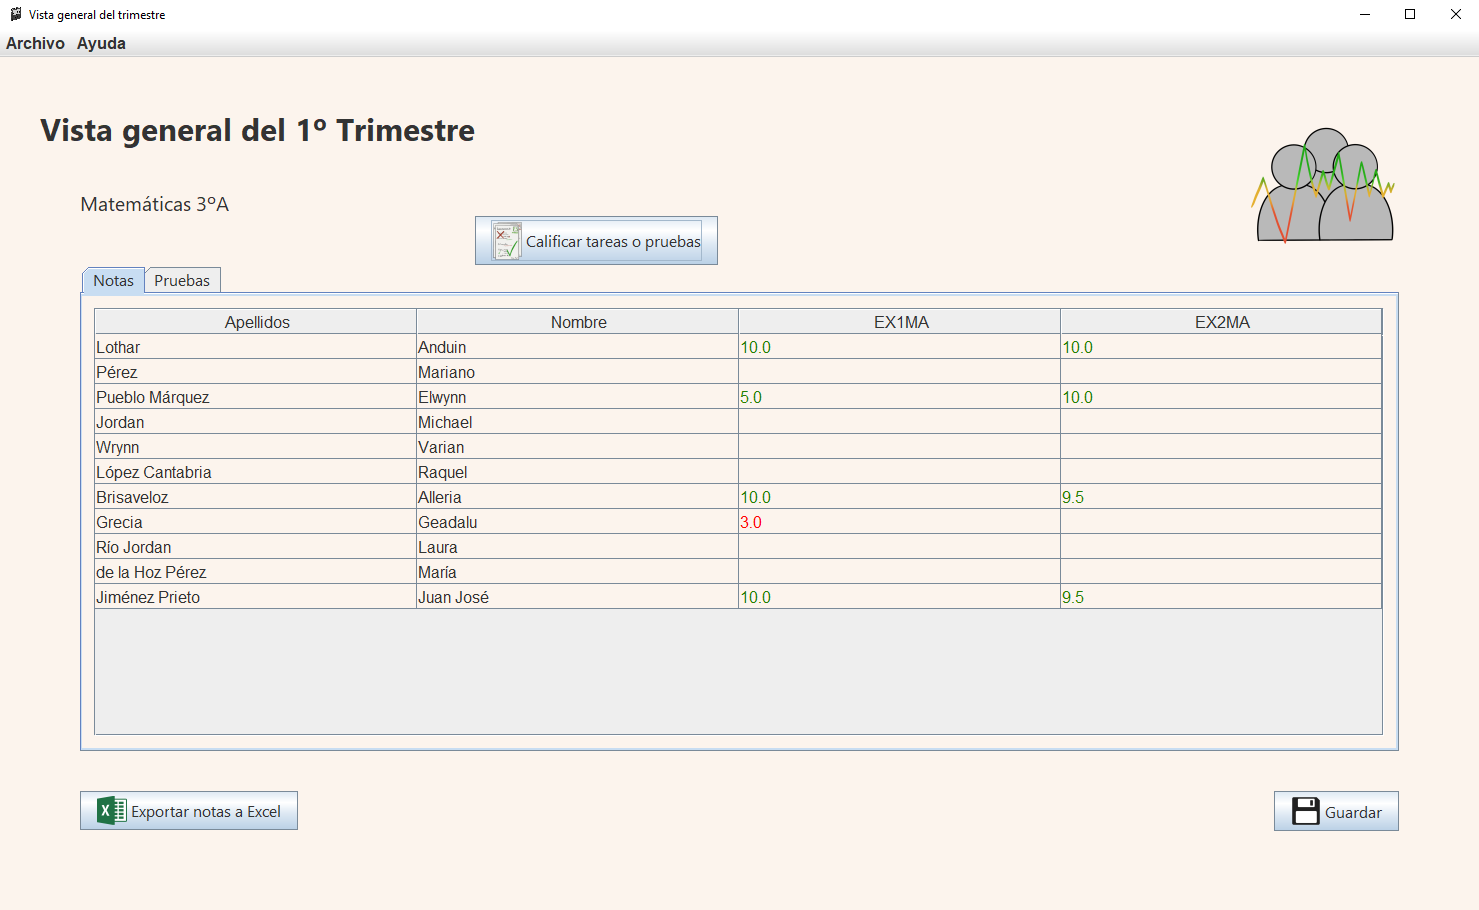
\includegraphics[width=1\linewidth]{figs/informetrimestre.png}
\caption{Primera pestaña de la ventana del informe por trimestre.}
\label{Fig:informetrimestre}
\end{figure}

Esta ventana está dividida, como hemos mencionado, en dos partes: la primera muestra una tabla informativa con todas las notas de las pruebas del trimestre elegido (ver figura \ref{Fig:informetrimestre}). En caso de que un alumno no tuviera que hacer la prueba, en la casilla saldría un guión '-'. 

\begin{figure}[H]
\centering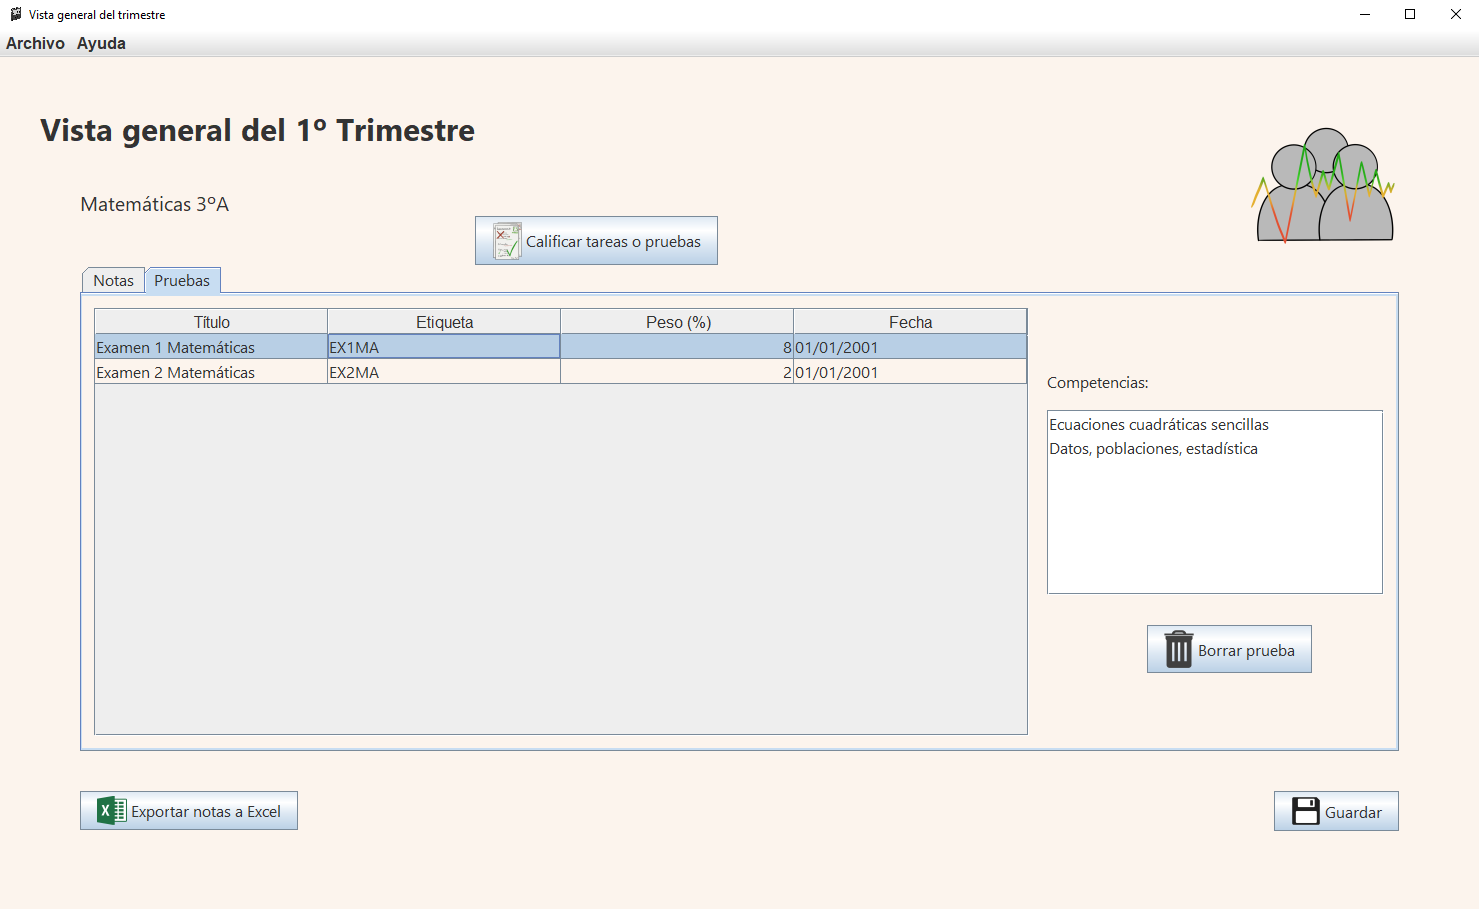
\includegraphics[width=1\linewidth]{figs/informetrimestre2.png}
\caption{Segunda pestaña de la ventana del informe por trimestre.}
\label{Fig:informetrimestre2}
\end{figure}

La segunda parte, accesible mediante la pestaña ''Pruebas'', presenta, en una tabla, los datos de las pruebas que se han introducido mediante el formulario de crear una nueva prueba, con posibilidad de edición (ver figura \ref{Fig:informetrimestre2}). Además, al seleccionar una prueba, a la derecha aparecerán las competencias asignadas a la misma y un botón para borrar la prueba del sistema, que borrará también las notas de los alumnos, si las tenían, y refrescará las dos tablas de la ventana.

\subsection{Manual de ayuda}
Existe un manual de ayuda, accesible por todas las ventanas desde el menú Ayuda>Manual de ayuda, que el usuario puede consultar en caso de duda sobre alguna funcionalidad.

Este manual se abre directamente por la página de la ventana desde la que se llama, y ofrece información detallada sobre lo que se puede hacer en cada ventana.

Se puede ver esta ventana en la figura \ref{Fig:ayuda}.

\begin{figure}[H]
\centering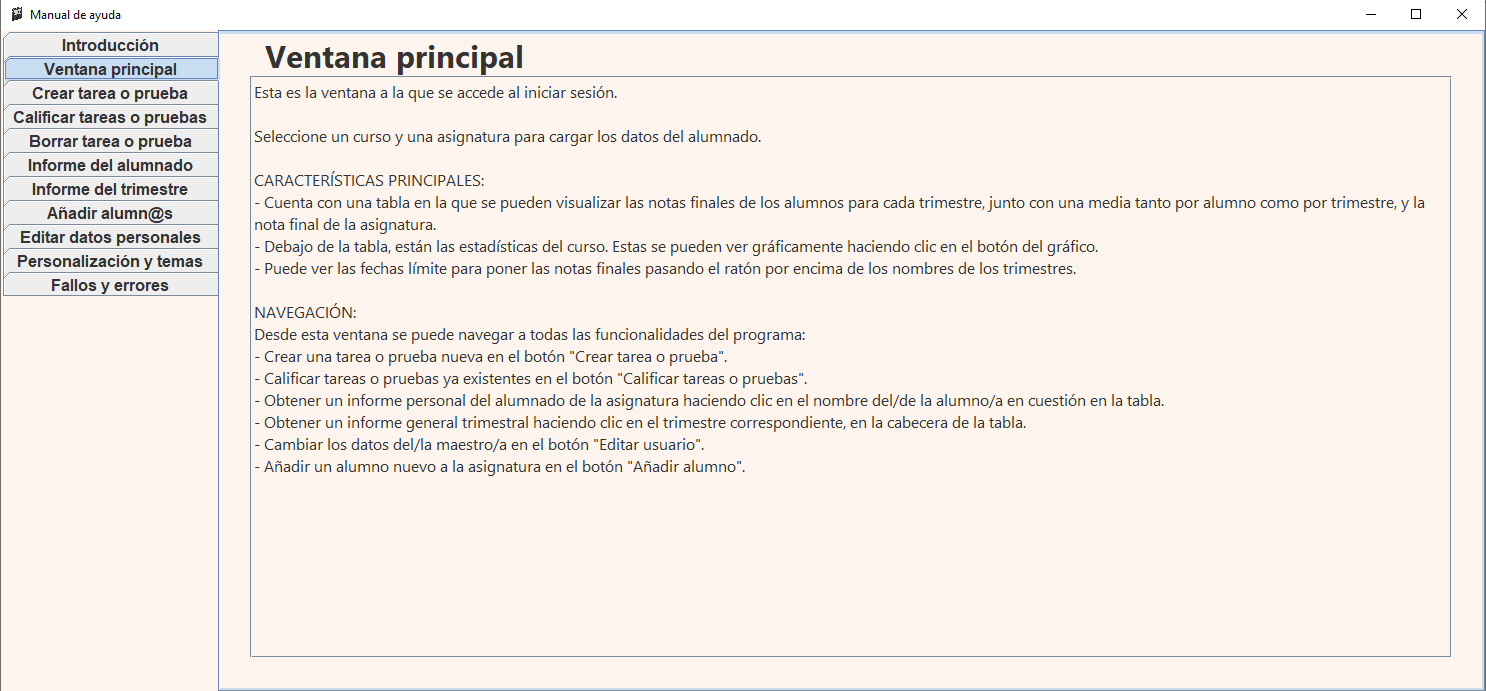
\includegraphics[width=1\linewidth]{figs/ayuda.png}
\caption{Ventana con el manual de ayuda.}
\label{Fig:ayuda}
\end{figure}